\chapter{Deep Latent Variables Generative Models}\label{ch:03}

\begin{remark}{Outline}
Among likelihood-based approaches for deep generative modelling, variational autoencoders (VAEs) offer scalable amortized posterior inference and fast sampling. However, VAEs are also more and more outperformed by competing models such as normalizing flows (NFs), deep-energy models, or the new denoising diffusion probabilistic models (DDPMs).
In this preliminary work, we improve VAEs by demonstrating how DDPMs can be used for modelling the prior distribution of the latent variables. The diffusion prior model improves upon Gaussian priors of classical VAEs and is competitive with NF-based priors.
Finally, we hypothesize that hierarchical VAEs could similarly benefit from the enhanced capacity of diffusion priors.
\end{remark}
\section{Prologue}
A word on the role of this part of the manuscript. Focus on the expressivity of deep probablistic models.

\subsection{Retrospective state of the art}

\paragraph{Variational auto-encoder}

\paragraph{Diffusion models}

\section{The paper: Diffusion Priors In Variational Autoencoders}

\subsection{Author contributions}

\subsection{Reading tips}

\subsection{Minor corrections}

\includepdf[pages=-]{papers/innf_latent_diffusion.pdf}

\section{Epilogue}
\subsection{Scientific impact}
\begin{figure*}
  \centering
  \begin{subfigure}[b]{.48\textwidth}
    \centering
    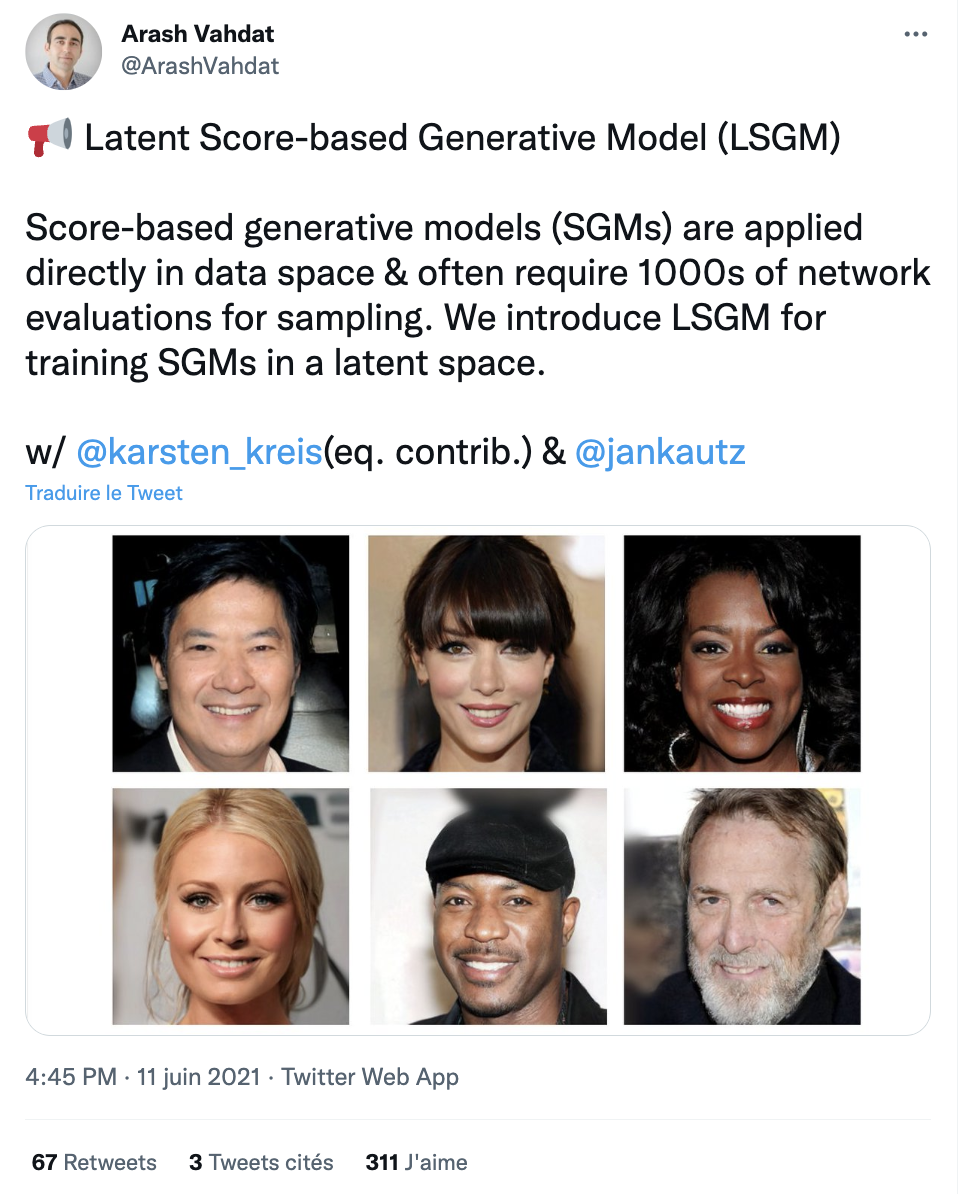
\includegraphics[width=.95\textwidth]{figures/impact_scholar/cont_diff_tweet.png}
    \caption{}
    \label{fig:cont_tweet}
  \end{subfigure}
  \begin{subfigure}[b]{.48\textwidth}
    \centering
    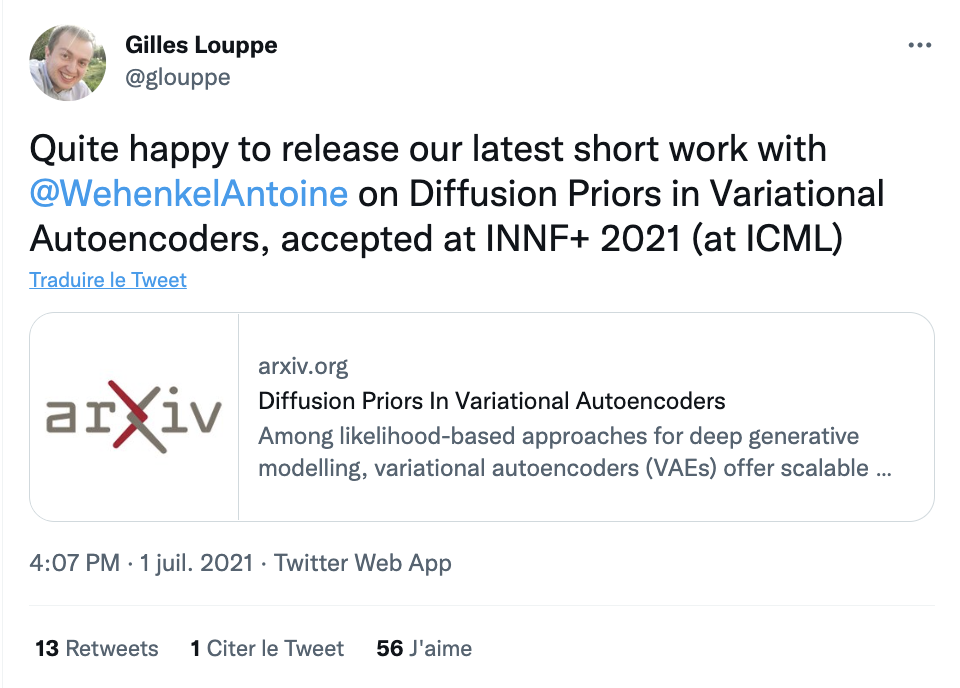
\includegraphics[width=.95\textwidth]{figures/impact_scholar/discret_diff_tweet.png}
    \caption{}
    \label{fig:discrete_tweet}
  \end{subfigure}
  \caption{Tweets advertising (\textbf{a}) The continuous-time diffusion models in the latent space from \citet{vahdat2021score} (\textbf{b}) The discrete-time diffusion models in the latent space from ours.}
\end{figure*}

As of July 2022, this article has received 5 citations according to Google Scholar since its publication in June 2021. We shall contrast this number with the 48 citations received by \citet{vahdat2021score} which was published in December 2021, at NeurIPS 2021 and was first released as a pre-print on Arxiv, in June 2021. Although the ideas expressed in the two papers are very similar, our work did not gain as much visibility as theirs. We acknowledge at least three fair reasons to explain this. First, publishing at NeurIPS brings much more visibility than at a workshop at ICML. This is natural as the reviewing process of NeurIPS is much stronger. Second, \citet{vahdat2021score} achieve state-of-the-art image synthesis by combining their idea with the right neural architectures, training tricks and computation power. In contrast, our work is a proof of concept and does not achieve state-of-the-art performance. In this regard, our work is preliminary compared to theirs. Finally, advertising science is arguably nowadays as important as science itself in machine learning.\citet{vahdat2021score} made a very good job as it can be seen by one tweet from the first author who advertised their paper in \Cref{fig:cont_tweet}. In contrast, Gilles Louppe advertised our paper on Twitter but it had $6\times$ smaller reach as it can be observed in \Cref{fig:discrete_tweet}.
\subsection{The practitioner's eye}

\subsection{What happened since then?}
- Work on continuous diffusion models and combining Enervy based models and VAES.
https://arxiv.org/pdf/2206.05895.pdf
- Diffusion models largely used for high fidelity image synthesis.
